\documentclass{article}
\usepackage[utf8]{inputenc}
\usepackage[english]{babel}
\usepackage{graphicx}
\usepackage{siunitx}
\usepackage{listings}
\usepackage{color}
\usepackage[toc,page]{appendix}
\usepackage[nottoc]{tocbibind}
\renewcommand{\appendixtocname}{Přílohy}
\renewcommand{\appendixpagename}{Přílohy}

\definecolor{mygreen}{rgb}{0,0.6,0}
\definecolor{mygray}{rgb}{0.5,0.5,0.5}
\definecolor{mymauve}{rgb}{0.58,0,0.82}

\lstset{
    language=SQL,
    keywordstyle=\color{blue},
    numbers=left,
    numbersep=5pt,
    numberstyle=\tiny\color{mygray},
    commentstyle=\color{mygreen},
    morekeywords={*, REPLACE, WITH, FUNCTION, RETURNS, BODY, DECLARE, RECORD, BEGIN, CONTINUE, PERFORM, RAISE NOTICE, NEW},
    stringstyle=\color{mymauve},
    breaklines=true,
    tabsize=2,
}
\lstset{literate=
  {á}{{\'a}}1 {é}{{\'e}}1 {í}{{\'i}}1 {ó}{{\'o}}1 {ú}{{\'u}}1
  {Á}{{\'A}}1 {É}{{\'E}}1 {Í}{{\'I}}1 {Ó}{{\'O}}1 {Ú}{{\'U}}1
  {à}{{\`a}}1 {è}{{\`e}}1 {ì}{{\`i}}1 {ò}{{\`o}}1 {ù}{{\`u}}1
  {À}{{\`A}}1 {È}{{\'E}}1 {Ì}{{\`I}}1 {Ò}{{\`O}}1 {Ù}{{\`U}}1
  {ä}{{\"a}}1 {ë}{{\"e}}1 {ï}{{\"i}}1 {ö}{{\"o}}1 {ü}{{\"u}}1
  {Ä}{{\"A}}1 {Ë}{{\"E}}1 {Ï}{{\"I}}1 {Ö}{{\"O}}1 {Ü}{{\"U}}1
  {â}{{\^a}}1 {ê}{{\^e}}1 {î}{{\^i}}1 {ô}{{\^o}}1 {û}{{\^u}}1
  {Â}{{\^A}}1 {Ê}{{\^E}}1 {Î}{{\^I}}1 {Ô}{{\^O}}1 {Û}{{\^U}}1
  {œ}{{\oe}}1 {Œ}{{\OE}}1 {æ}{{\ae}}1 {Æ}{{\AE}}1 {ß}{{\ss}}1
  {ű}{{\H{u}}}1 {Ű}{{\H{U}}}1 {ő}{{\H{o}}}1 {Ő}{{\H{O}}}1
  {ç}{{\c c}}1 {Ç}{{\c C}}1 {ø}{{\o}}1 {å}{{\r a}}1 {Å}{{\r A}}1
  {€}{{\euro}}1 {£}{{\pounds}}1 {«}{{\guillemotleft}}1
  {»}{{\guillemotright}}1 {ñ}{{\~n}}1 {Ñ}{{\~N}}1 {¿}{{?`}}1
}

\rmfamily

\begin{document}

\begin{titlepage}
		
\includegraphics[width=300px]{fav_logo.pdf}\par
		\vspace{1cm}
		\centering
		{\scshape\LARGE Západočeská univerzita \par}
		\vspace{0.5cm}
		{\scshape\Large Fakulta aplikovaných věd \par}
		\vspace{2cm}
		{\Large\bfseries Semestrální práce předmětu KIV/DB2 \par}
		\vspace{0.5cm}
		{\Large Hledání min \par}
		\vspace{0.5cm}
		{\Large\itshape Petr Štechmüller\par}
		\vfill
		{\large \today\par}
\end{titlepage}

\tableofcontents

\newpage 

\section{Zadání}
Cílem této semestrální práce je implementovat hru "hledání min"
čistě v databázové vrstvě.
Aplikace umí:
\begin{itemize}
    \item Vytvořit novou hru (předdefinovanou i vlastní)
    \item Zobrazit herní pole
    \item Označit minu
    \item Zobrazit vyhrané i prohrané hry
    \item U prohrané hry zobrazit špatně označené miny
\end{itemize}

\section{Datová analýza}
Datový model je k dispozici v příloze \ref{fig:era}.

\section{Funkční analýza}
V této sekci budu demonstrovat zajímavé části kódu.
První ukázka kódu \ref{lst:vitezove} obsahuje kód pro pohled s vítěznými hrami.
V pohledu zobrazuji sloupečky: id hry, id oblasti, doba hrani, počet řádků, počet sloupců,
celkový počet min a obtížnost. Doba hraní se vypočítá jako rozdíl mezi prvním
a posledním tahem. To jsem realizoval pomocí rozdílu dvou SELECTů.

\begin{minipage}{\linewidth}
\lstinputlisting[language=SQL, caption={Pohled Vítězové}, label={lst:vitezove}]{code/vitezove.sql}
\end{minipage}


Druhá ukázka pohledu \ref{lst:chybne_miny} se zaměřuje na kód pro zobrazení chybně označených min.
Rozhodl jsem se, že chybné miny se budou zobrazovat pouze u her, které již byly neúspěšně
dohrány. To zajišťuje podmínka \lstinline{hra.id_stav = 3}.

\begin{minipage}{\linewidth}
\lstinputlisting[language=SQL, caption={Pohled Chybné miny}, label={lst:chybne_miny}]{code/chybne_miny.sql}
\end{minipage}

Třetí ukázka kódu \ref{lst:odkryj_pole} se zaměřuje na proceduru, 
konkrétně \textit{odkryj pole}. Tato procedura slouží k rekurzivnímu odkrytí pole, 
na kterém se nenachází žádná mina. 
Tato procedura je volána z triggeru \ref{lst:zpracuj_po_oznaceni_tahu}, 
který se aktivuje vždy po vložení záznamu \ref{lst:spust_po_oznaceni_tahu} 
do tabulky \textit{TAH}.

\begin{minipage}{\linewidth}
\lstinputlisting[language=SQL, caption={Funkce triggeru, která je zavolána
pro každý vložený řádek do tabulky tah},
label={lst:zpracuj_po_oznaceni_tahu}]{code/zpracuj_po_oznaceni_tahu.sql}
\end{minipage}

\begin{minipage}{\linewidth}
\lstinputlisting[language=SQL, caption={Trigger, který se aktivuje po vložení záznamu do tabulky tah},
label={lst:spust_po_oznaceni_tahu}]{code/spust_po_oznaceni_tahu.sql}
\end{minipage}

\section{Scénáře}
Na následujících řádcích uvedu příklady, jak lze hru hrát.

\subsection{Nová hra}
Hru lze založit dvěma způsoby. Buď si uživatel vybere již předpřipravenou
velikost herního pole, nebo si vytvoří vlastní velikost.
Příkaz pro vytvoření nové hry je vidět v kódu \ref{lst:new_game}.

\begin{minipage}{\linewidth}
\lstinputlisting[language=SQL, caption={Nová hra},
label={lst:new_game}]{code/new_game.sql}
\end{minipage}

\subsection{Zobrazení herního pole}
Kdykoliv v průběhu hry si lze zobrazit herní pole příkazem \ref{lst:oblast_tisk}.
Přákaz vrátí tabulku která obsahuje následující znaky:
\begin{itemize}
    \item ? - neodkryté pole
    \item + - označená mina
    \item 0-8 - počet min v okolí aktuálního pole
\end{itemize}

\begin{minipage}{\linewidth}
\lstinputlisting[language=SQL, caption={Nová hra},
label={lst:oblast_tisk}]{code/oblast_tisk.sql}
\end{minipage}

\subsection{Vložení tahu}
Pro vložení tahu slouží příkaz \ref{lst:vloz_tah}.
Při pokusu vložit stejný tah vícekrát bude uživatel
upozorněn chybovou hláškou, že tah již byl vložen.


\begin{minipage}{\linewidth}
\lstinputlisting[language=SQL, caption={Vložení tahu},
label={lst:vloz_tah}]{code/vloz_tah.sql}
\end{minipage}

\subsection{Označení miny}
Minu je možné označit příkazem \ref{lst:oznac_minu}.
Pokud je příkaz zavolán znovu, v daném poli se zruší označení miny.

\begin{minipage}{\linewidth}
\lstinputlisting[language=SQL, caption={Označení miny},
label={lst:oznac_minu}]{code/oznac_minu.sql}
\end{minipage}

\section{Klientská část}
Klientská část vznikla primárně z důvodu mé lenosti zadávat jednotlivé
příkazdy ručně. Snažil jsem se o co nejjednodušší řešení, které by 
co nejlépe pokrylo potřeby uživatele. 
Klient je rozdělen na dvě části: frontend a backend.
\subsection{Backend}
Serverová část pro klientskou aplikaci je jenom taková mezivrstva starající se o komunikaci
mezi webovou aplikací a databázi. Server je napsaný v JavaScriptu v prostředí NodeJS.
\subsection{Frontend}
Webová aplikace je psána v TypeScriptu a je postavena na frameworku Angular 5.
Díky Angularu byla aplikace velice rychle vytvořena.
O komunikaci mezi frontendem a backendem se stará websocket.
Při načtení webové aplikace se vytvoří trvalé spojení, po kterém se aktivně transportují
data jak z klienta na server, tak i opačným směrem. Nejde tedy o klasickou komunikaci
dotaz - odpověď. Díky této technologii jsem si mohl dovolit vytvořit uživatelsky přívětivou
aplikaci bez obnovování stránky.
V příloze jsou k dispozici náhledy z webové aplikace.
\subsection{Spuštění aplikace}
Každá webová aplikace potřebuje být spuštěna na nějakém serveru.
Pro zpřístupnění kientské části je potřeba mít nainstalovaný NodeJS server.
Server se spustí příkazem \lstinline{npm start}.
Klient potrebuje také spustit server a to příkazem \lstinline{npm run-script build}.
Nakonec stačí spustit prohlížeč na adrese stroje s portem 4200 například 
\lstinline{localhost:4200}.
Nastavení přístupových údajů k databázi se provádí v souboru \textit{sio/index.js}.
Na začátku tohoto souboru se nachází objekt \textbf{settings}, který obsahuje přístupové
údaje k databázi.

\newpage

\section{Závěr}
Aplikace splnila všechny body zadání a je doplněna o přívětivé uživatelské rozhraní.
Během testování jsem zjistjil, že pokud vygeneruji příliš veliké pole (100x100) s jednou
minou, tak databáze nezvládne vložit tah, protože dotaz "umře" na přetečení zásobníku.
Při programování jsem velim často navštěvoval stránku PostgreSQLTutorial \cite{postgres},
která obsahuje velké mnoství užitečných tipů a návodů jak tvořit funkce a triggery v
databázi PostgreSQL.

\medskip
\bibliographystyle{unsrt}
\bibliography{reference}

\newpage

\begin{appendices}
\section{Procedura odkryj pole}
\lstinputlisting[language=SQL, label={lst:odkryj_pole}]{code/odkryj_pole.sql}

\newpage
\section{Datový model databáze}
\begin{figure}[!h]
\begin{center}
    \fbox{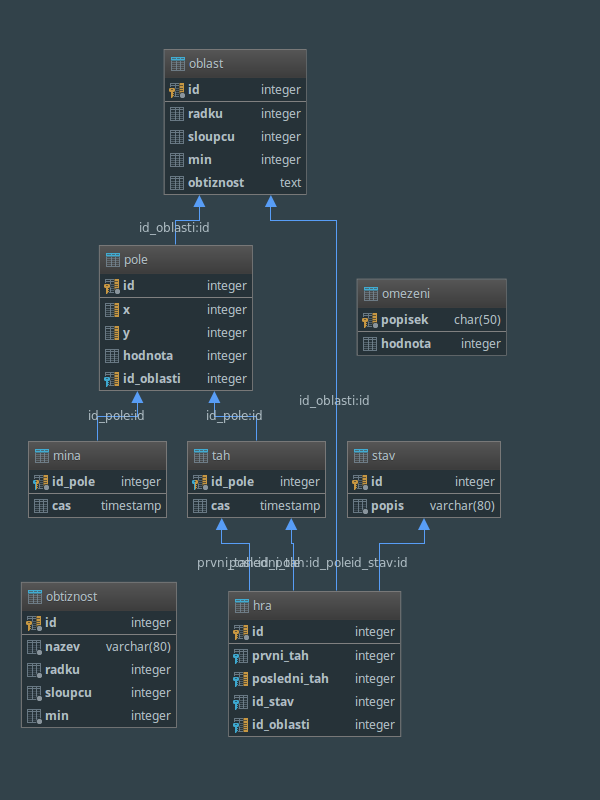
\includegraphics[width=\linewidth]{img/era.png}}
    \caption{Datový model databáze}
    \label{fig:era}
\end{center}
\end{figure}

\newpage
\section{Ukázka klientské aplikace}
\begin{figure}[!h]
\begin{center}
    \fbox{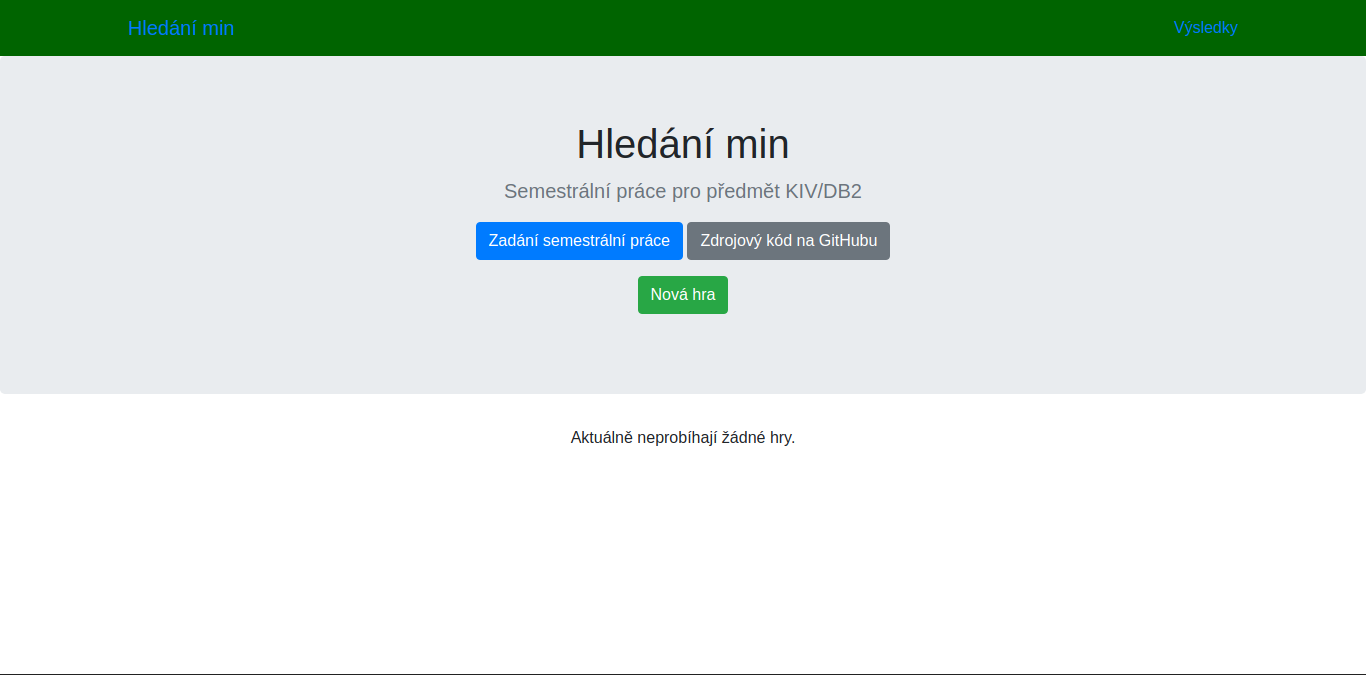
\includegraphics[width=\linewidth]{img/overview.png}}
    \caption{Hlavní stránka aplikace}
    \label{fig:overview}
\end{center}
\end{figure}

\begin{figure}[!h]
\begin{center}
    \fbox{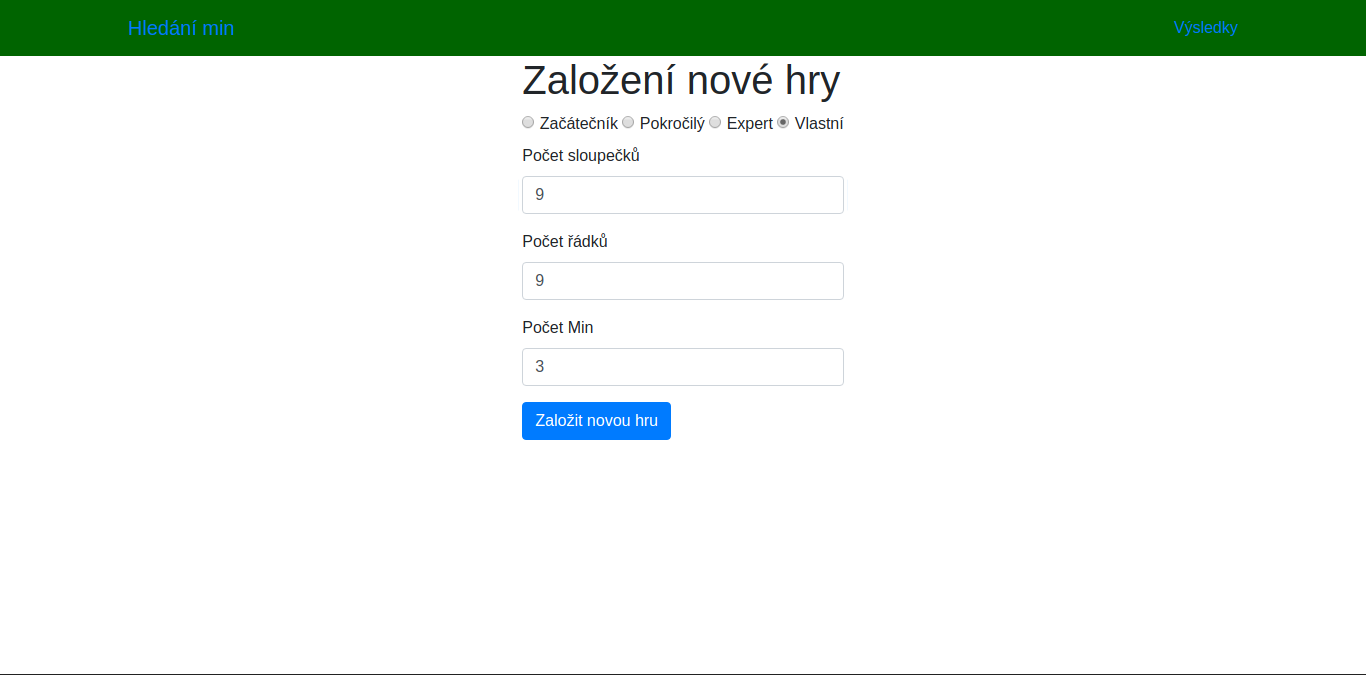
\includegraphics[width=\linewidth]{img/create_game.png}}
    \caption{Formulář pro založení nové hry}
    \label{fig:new_game}
\end{center}
\end{figure}

\begin{figure}[!h]
\begin{center}
    \fbox{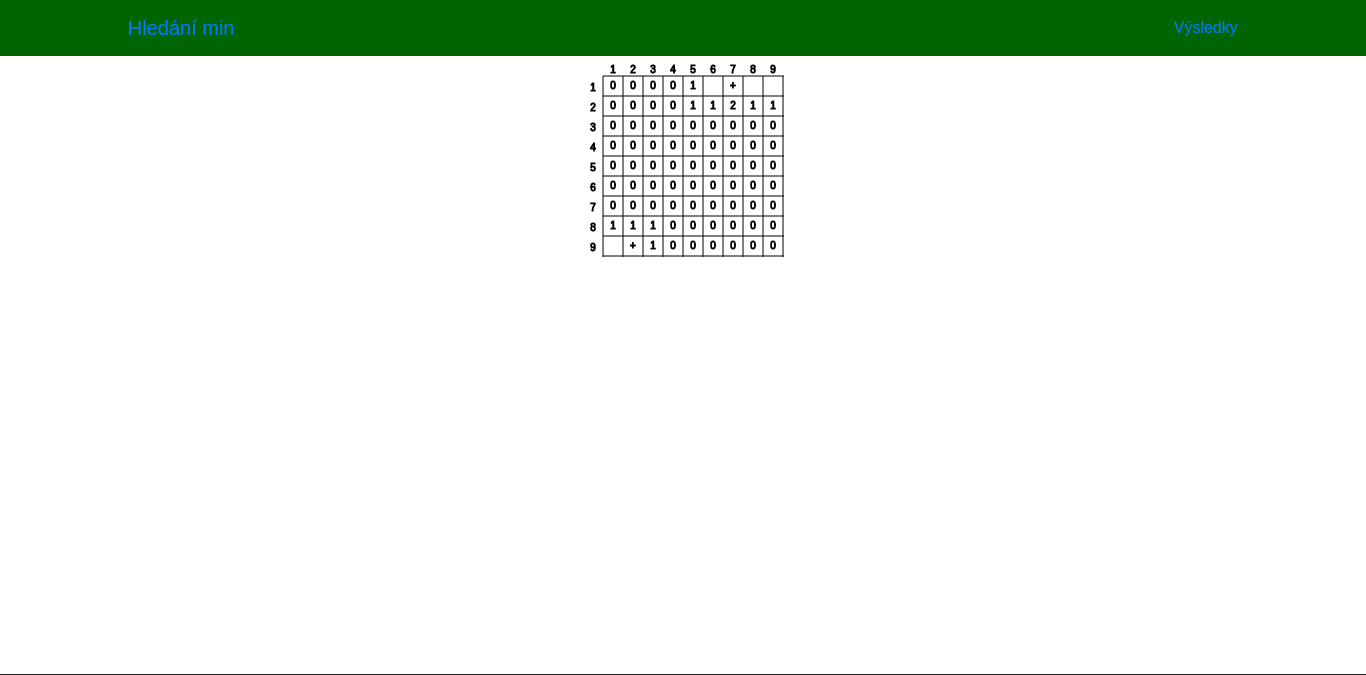
\includegraphics[width=\linewidth]{img/game.png}}
    \caption{Rozehraná hra}
    \label{fig:game}
\end{center}
\end{figure}

\begin{figure}[!h]
\begin{center}
    \fbox{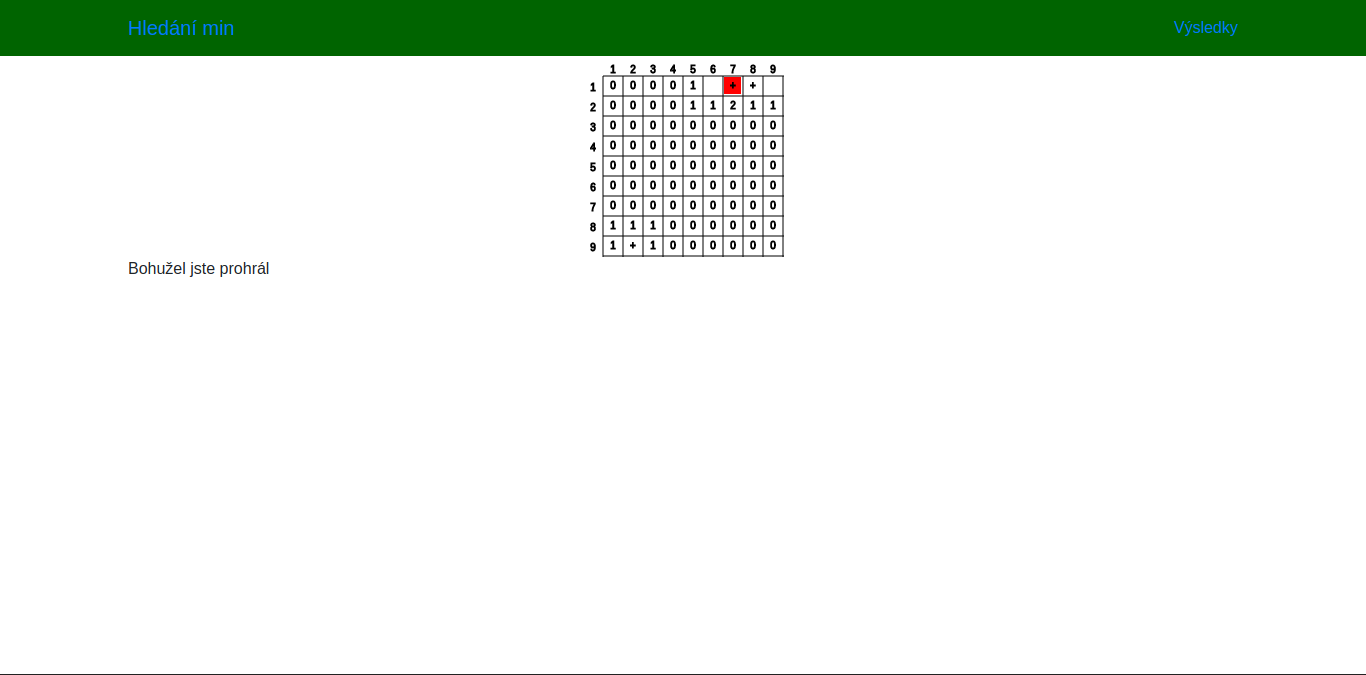
\includegraphics[width=\linewidth]{img/loose.png}}
    \caption{Prohraná hra se špatně označenými minami}
    \label{fig:loose}
\end{center}
\end{figure}

\begin{figure}[!h]
\begin{center}
    \fbox{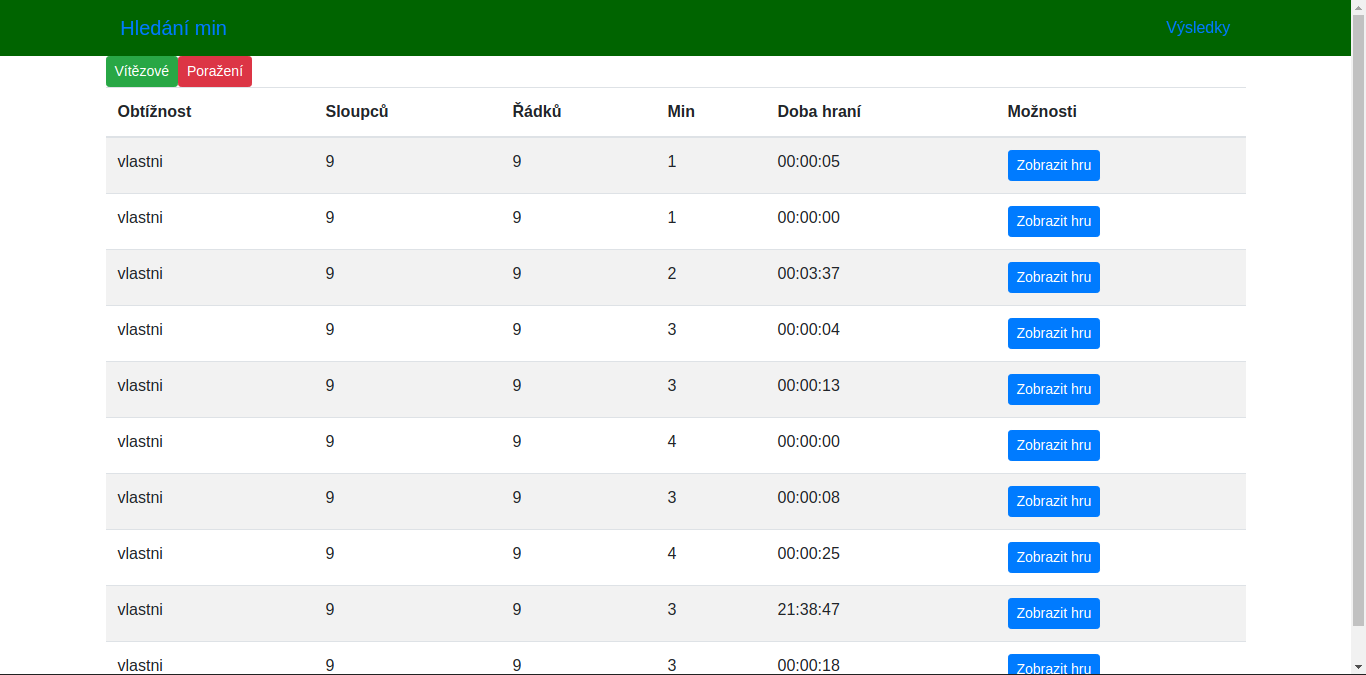
\includegraphics[width=\linewidth]{img/scoreboard.png}}
    \caption{Výsledková listina}
    \label{fig:scoreboard}
\end{center}
\end{figure}

\end{appendices}



\end{document}
